\documentclass[10pt,twocolumn,letterpaper]{article}

% \usepackage{cvpr}              % To produce the CAMERA-READY version
\usepackage[pagenumbers]{cvpr} % To force page numbers, e.g. for an arXiv version

% Include other packages here, before hyperref.
\usepackage{graphicx}
\usepackage{comment}
\usepackage{amsmath}
\usepackage{amssymb}
\usepackage{booktabs}
\usepackage[toc,acronym]{glossaries}
\newacronym{AI}{AI}{Artificial Intelligence}
\newacronym{APC}{APC}{Autoregressive Predictive Coding}
\newacronym{CLI}{CLI}{Console Line Interface}
\newacronym{DL}{DL}{Deep Learning}
\newacronym{DQN}{DQN}{Deep Q Network}
\newacronym{DRL}{DRL}{Deep Reinforcement Learning}
\newacronym{GMM}{GMM}{Gaussian Mixture Models}
\newacronym{GPU}{GPU}{Graphical Processing Unit}
\newacronym{HPC}{HPC}{High Performance Computing}
\newacronym{InfoNCE}{InfoNCE}{Information Noise-Contrastive Estimation}
\newacronym{LSCC}{LSCC}{Lung Squamous Cell Carcinoma}
\newacronym{MOCO}{MOCO}{Momentum Contrast for Unsupervised Visual Representation Learning}
\newacronym{NLDL}{NLDL}{Northern Lights Deep Learning}
\newacronym{NLP}{NLP}{Natural Language Processing}
\newacronym{NRIS}{NRIS}{Norwegian Research Infrastructure Services}
\newacronym{RL}{RL}{Reinforcement Learning}
\newacronym{SSL}{SSL}{Self-Supervised Learning}
\newacronym{TCGA}{TCGA}{The Cancer Genome Atlas}
\newacronym{TD}{TD}{Temporal Difference}
\newacronym{UMAP}{UMAP}{Uniform Manifold Approximation and Projection}
\newacronym{WSI}{WSI}{Whole Slide Image}
\newacronym{XAI}{XAI}{Explainable AI}
\newacronym{tf-idf}{tf-idf}{term frequency-inverse document frequency}
\newacronym{CDR}{CDR}{Clinical Data Resource}
\newacronym{CPTAC}{CPTAC}{Clinical Proteomic Tumor Analysis Consortium}


\usepackage[pagebackref,breaklinks,colorlinks]{hyperref}
\usepackage[capitalize]{cleveref}
\crefname{section}{Sec.}{Secs.}
\Crefname{section}{Section}{Sections}
\Crefname{table}{Table}{Tables}
\crefname{table}{Tab.}{Tabs.}

\def\cvprPaperID{*****}
\def\confName{NLDL}
\def\confYear{2023}

% TODO Cite presentations?

\begin{comment}
The written report should be 8 pages in length (double column, excl. references). To standardise things, please use the CVPR formatThe report should include both a short summary of the material covered (approx. 4 pages) and a description of the solution to a practical component.

Remember that the first four pages of your final report should cover aspects from all tutorials (not only focusing on the one relevant for the practical task)

Topics covered:
A gentle introduction to Deep Reinforcement Learning

Self-Supervised Learning: Training Targets and Loss Functions

The Challenge of Unverfiability in eXplainable AI Evaluation

Data representativity and low-resource modeling in deep learning

High Performance Computing for Deep Learning

Representation learning and learning with few data

\end{comment}

% if lacking text, write about the presentors (https://www.nldl.org/winter-school)

\begin{document}
\title{NLDL Winter School 2023}

\author{Anders Sildnes\\
University of Tromsø\\
Postboks 6050 Langnes\\
{\tt\small anders.sildnes@uit.no}
}
\maketitle
% Computational pathology is study of disease using methods such as artificial intelligence. For building models, there are three main hindrances: 1) lack of publicly available data, 2) large image-size and high number of details and 3) lack of ground truth data due to expert disagreeance. Consequently, developers have to compromise when building a model. To know if models are accurate enough, explainable AI can help. But, are the explanations good enough that a pathologist can trust a model used to evaluate patient diagnosis and/or prognosis? 


\section{Introduction} \label{sec:intro}
This is a report from the 2023 Northern Lights Deep Learning (NLDL) conference. The first four pages contains a summary from each of the topics covered Monday 9th of January and Friday 13th January. I have primarily used the presentations as a source, but supplemented a little with papers I have found online. Citations to these sources are given. 
I have omitted some content from all the presentations to adhere to the length requirements. A detailed programme can be found on the website: \href{https://www.nldl.org/winter-school}{https://www.nldl.org/winter-school}. 
% To make the first four pages I have followed each of the presentation slides and supplemented with extra information found in other sources, which of course are cited.
% if need be, summarize my findings here

\section{Deep Reinforcement Learning}\label{sec:drl}
\begin{comment}
  \gls{RL} has emerged as a powerful technique in modern machine learning, allowing a system to learn through trial and error. We will introduce some fundamental principles upon which this family of methods is based. In the first part, we give a summary of classical reinforcement learning and thus provide the essentials for understanding Deep Reinforcement Learning (DRL). In the second part, we shift the focus onto DRL and look at how deep learning enhances classical reinforcement learning, leading to powerful new algorithms. These algorithms include DQN playing Atari games at a superhuman level, PPO solving robot locomotion problems, and Alpha Zero learning to play GO, Chess, and Shogi. In the limited time of such a mini-tutorial, we can of course only sketch the main characteristics, but we intend to motivate to look deeper into this fascinating family of methods.
\end{comment}
\gls{RL} is a branch of AI. One or more agents interact with a given environment and teach themselves 
behaviours that maximize a goal-function. Often this relies a great number of iterations; e.g. AlphaGo Zero played 4.9 million rounds of Go with itself before being released~\cite{goWithoutHumans}. This got news coverage all over the world as Go had long been considered to be a game too complicated for computers.

\gls{RL} agents operates in discrete time. At each timestep $t$ the agent observes its environment. Each observation $O_{t}$ modifies the agent state $s_{t}$, a processed representation to the history of events. Based on $s_{t}$ the agent chooses it's action $A_{t}$. The choice is made by choosing the action thought to maximize the reward $R_{t}$ of the agent in the future (next state). The expected return from the eyes of an agent is measured by it's goal function $G_{t}$, being the sum $G_{t} = \sum_{k=t+1}^{\inf{}}{R_{k}}$.
A problem with this goal function is that the agent can get stuck. E.g. in a dead end of a labyrinth; refusing to take a step back to find another path to the goal. A discount factor, noted $\gamma{}$, ensures that rewards less valuable over time, typically modelled as $G_{t} = \sum_{k=t+1}^{\inf{}}\gamma^{k}{R_{k}}$ (which can also be expressed a recursive $R_{t+1} + \gamma{G_{t+1}}$). Hence, if you stick in a dead end for too long, it doesn't pay off, and any other path that penultimately gets to another reward faster is better. The use of discount factors in reward functions is referred to as \textit{\gls{TD} learning}.

But how is the reward chosen? Each state is given a \textit{value function}. This is the expected value from being in a state $s$: $V_{\pi} = \mathbb{E}_{\pi} [ G_{t} | s = s_{t}]$. $\pi$ is here defined as the policy for what action to choose. Usually we cannot know exactly what the outcome of an action is, therefore we model actions by stochastic policies $\pi{}(a | s)$ which gives likelyhood of future actions. An example is a robot taking a step forward, but sliding on a banana peel and consequently falling. This lesson means that re-visiting the same state later in the future should not yield the same action, even if the policy is the same. The same does not apply to e.g. chess, where we can set a deterministic policy since we know exact outcomes from actions (moving pieces). 
Analogous to the value function is the action value: $q_{\pi{}} = \mathbb{E} [ G_{t} \vert{} S_{t} = s \cap A_{t} = a]$. This function (as given here) is strict to the policy $\pi$, i.e., in order to predict the future value of actions, you have to stay with the same $\pi$. The \textit{q} is often referred to as \textit{quality}. 


% To resolve which future state that is desirable, the Bellman equation~\cite{bellman} is often used.
% It sums over all possible state successor states $s'$ and evaluates their estimated values given policy $\pi{}$ and probabilistic expection $p(s', r \vert{} s, a)$. It's full formal notation is given in~\Cref{eq:bellman}:
% \begin{equation}\label{eq:bellman}
%   V_{\pi}(s) = \sum_{a}{\pi(a\vert{}s})\sum_{s'}\sum_{r}{p(s', r \vert{} s, a) * [r + \gamma * v_{\pi{}}(s')]}
% \end{equation}

Keeping a mapping between states and their expected values can be exhaustive for computer memory. Finding the right policy can also be difficult. If we think of neural network for what they are, \textit{function approximators}, it seems intuitive to use them for approximating the value function and/or action policy. This helps us resolve the problem of finite available space in action-value mappings. Hence, the field of \textbf{\gls{DRL}} emerges. There are several examples already of popular tools/models built with \gls{DRL}, such as AlphaTensor~\cite{alphaTensor} for matrix multiplication, DeepNash~\cite{stratego} for the game of Stratego, etc. 

The neural nets in \gls{DRL} (a.k.a \gls{DQN}) lacks ground truth, but rather rely on rewards for optimization. The problem is that these rewards may come at delayed moments or at the influence of unknown variables. This is essentially noise in the learning loop. Therefore, there are several techniques used in conjuction with the neural nets to improve their accuracy. One such trick is experience replay: steps are recorded with $(s_{t}, a_{t}, s_{t+1}, r_{t})$ in a replay buffer. Now, whenever we perform an action, we can learn not only from the change in environment, but we may use extra samples from past events.

% Talk more about policy gradients?

So far in this summary the \gls{RL} approaches have been \textit{model-free}: to learn of the world, actions are performed and evaluated. The alternative is \textit{model-based} \gls{RL}, wherein the agent can plan ahead by making predictions about how actions affect the world: $p(s_{t+1} \vert{} s_{t}, a_{t})$. The advantage of model-based \gls{RL} is primarily it's sample efficiency since we can prune away more actions during the learning phase. This is the case of Alpha Zero~\cite{alphaZero}. There have, however, been other strides in e.g. MuZero~\cite{muZero}, which can also train its own model to be used by \gls{RL} to predict future actions.

% The bellman equation is commonly used to asses a state value.

% This is often a greedy process where short-term benefits are prioritized over long-term benefits, similar to laws of finance, future gains are discounted. 


% \gls{RL} is sequential, i.e. future actions depend on previous ones. Unlike 


% TODO: Ai gyms?

\section{Self Supervised Learning}\label{sec:ssl}
\begin{comment}
Humans learn much under supervision but even more without. Such will apply to machines. Self-supervised learning is paving the way by leveraging unlabeled data which is vastly available. In this emerging learning paradigm, deep representation models are trained by supervised learning with supervisory signals (i.e., training targets) derived automatically from unlabeled data itself. It is abundantly clear that such a learnt representation can be useful for a broad spectrum of downstream tasks with the need of significantly less supervised data.

As in supervised learning, key considerations in devising self-supervised learning methods include training targets and loss functions. The difference is that training targets for self-supervised learning are not pre-defined and greatly dependent on the choice of pretext tasks. This leads to a variety of novel training targets and their corresponding loss functions. This tutorial aims to provide an overview of training targets and loss functions developed in the domains of speech, vision and text. Further, we will discuss some open questions, e.g., transferability, and under-explored problems, e.g., learning across modalities. For example, the pretext tasks, and thus the training targets, can be drastically distant from the downstream tasks. This raises the questions like how transferrable the learnt representations are, how to choose training targets and how to explore representations. We will also discuss the link between semi-supervised and self-supervised learning.
\end{comment}
There are now four different training paradigms in machine learning. 1) is supervised learning, in which an annotator labels data to be used by a machine learning model. 2) is semi-supervised, which can combine unlabeled data and labelled data together. 3) is then unsupervised learning and then 4) self-supervised, in which the model is able to make labels on its own. Approach 1 and 2 both depend on annotations which may be costly (and tedious) to aquire and approach 3 is fast but has limited learning capacity. \gls{SSL} is intending to resolve the headaches from the former 3. The labels have to be introduced \textit{at some point}, but \gls{SSL} can be used as a \textit{pretext} task. \gls{SSL} has made big advancements in \gls{NLP}, for example in the most recent ChatGPT (made by OpenAI~\cite{openAI}) (albeit its underlying model based on GPT-3 also uses other techniques~\cite{gpt3}).

For speech and text, one technique to make \gls{SSL} efficient is \gls{APC}~\cite{chung2020generative}. This technique relies on encoding context in the form of past elements into a latent space (a model's interpretation) in order to predict future elements. This prediction is made using a softmax-layer which effectively calculates the probability of future tokens (referred to as frames). The loss function of the model also uses the probability of past and future frames as an optimizer. The difficulty of this approach is having enough computer memory to store all the past tokens. To aid this it is helpful to use \textit{transformers}, which have attention-based learning and may compress some of past frames. This could e.g. be elimiting noise in audio sounds.

Since \gls{SSL} only defines \textit{pretext} tasks, it does mean that results from \gls{SSL} may not be transferrable to other domains or objects. For example, data2vec (CITE), another \gls{SSL} technique for \gls{NLP}, relies on having contextualized training targets to learn the embedding of words and documents. I.e. by calculating a \gls{tf-idf} from carefully selected documents it is able to calculate a good word embedding to be used in later analysis. For non-related domains the \gls{tf-idf} would be off, however. 
% TODO: compare program's description of talks vs what I have written



\section{Unverfiability in eXplainable AI Evaluation}\label{sec:xai}
\begin{comment}
  In recent years, the interest in \gls{XAI} techniques has undoubtedly exploded and countless methods and toolboxes are now at the disposal of \gls{XAI} researchers, ML practitioners and data scientists alike. Despite my shared enthusiasm for this productive development, until recently, the topic of \gls{XAI} evaluation was grossly understudied — and caused confusion about which explanation methods work and under what conditions. In this tutorial, we will take an in-depth look at some of the most recent developments in \gls{XAI} evaluation and review the solutions that the community has put forward to circumvent the fundamental problem of \gls{XAI} — the lack of ground-truth explanations. In addition to this, we will discuss The Challenge of Unverfiability — why evaluation is so difficult to get right (and what we can do about it). At the end of the tutorial, a brief yet hands-on introduction to Quantus will be given, which is an open-source library intended for \gls{XAI} researchers to evaluate local neural network explanations.
\end{comment}
\gls{DL} depends on several hidden layers that can have millions of billions of neurons. These neural nets are therefore often regarded as a ``black box'' because it is difficult to get an overview of how they make their predictions. Understanding how a model works may be important, especially if the model is going to be used in critical settings such as medicine or any kind of hazard detection. 

\gls{XAI} aims to resolve these issues. \gls{XAI} not only increases our trust in how \gls{AI} models work, they can unravel biases and generate new insights. If you for example want an \gls{AI} to separate dogs and wolves, it might be that the \gls{AI} is learning to recognize the background setting, which for wolves will more often be outside in the woods. It might also be that a model picks up artifacts in photos not seen or known to humans that are nevertheless relevant. 

A technique for \textit{explainability} is to occlude parts of inputs. If the model is still able to accurately predict the classification, that means that the relevant features are still in the photo. You can repeat this process to retain only the features that the model depends on. A technique for \textit{comprehension} is mapping model outputs to a three-dimensional or two-dimensional space (covered in TODO CREF later) to visualize how a model maps different features. If two (theoretically) similar inputs don't end up close to each other, this could then be an \gls{XAI} relevant insight.

Methods like data occlusion is \textit{model agnostic}: even if you modify or change the model the method would still operate in the same way. There is another family of techniques that are \textit{model aware}. One such method is saliency mapping~\cite{simonyan2014deep}, a gradient-based method. Somewhat similar to data occlusion, input to a machine learning model is modified. This time, however, the output from the model is tracked to determine its gradient with each change. By tracking what regions impact the gradients the most, the most relevant regions are established. The downside with model-aware methods is that their dependency of the model, and if the model is unstable, the explanations may be unstable, too.

But, how robust are the metioned explanations?~\cite{geometryToBlame} finds that it is possible to modify input images in a way that is (barely) unoticable to humans but nevertheless dramatically modifies the output explanations. One such pertubation is shown in~\Cref{fig:arbitrary}.

Since explanations can be erroneous and frail, a tool to measure the quality of explanations seems called for. I discuss this more in detail in~\Cref{sec:quantifiable}.

\begin{figure}
  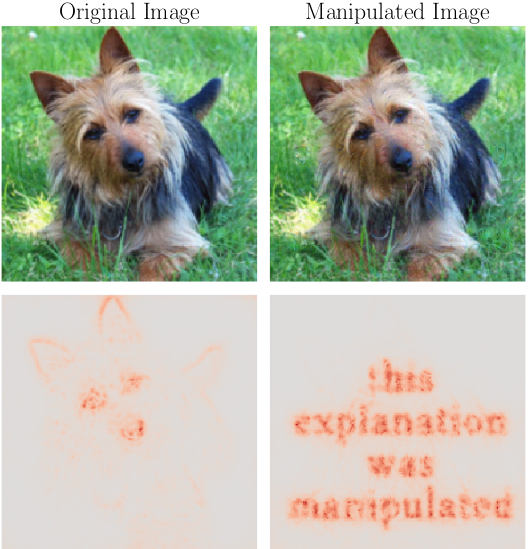
\includegraphics[scale=.4]{./manipulated_explanation_ai.png}
  \caption{Left side: original image with its explanation. Right side is a seemingly similar image, but it is modified in such a a way that the explanation output is completely different. The figure is taken from~\cite{geometryToBlame}}
\label{fig:arbitrary}
\end{figure}


% can write about local vs global methods, or just include that

\section{Data representativity and low-resource in Deep Learning}\label{sec:representative}
\begin{comment}
This tutorial first introduces data representativity in artificial intelligence and machine learning, in particular how to measure data representativity and construct datasets that are fair and unbiased in contrast to datasets that work best on average. Secondly, we look at semi-supervised learning and transfer learning for low-resource applications, including a variational autoencoder for speech. The two parts consider robustness towards distribution shifts from a data and a modelling perspective.
\end{comment}
\gls{DL} depends on many iterations with data to improve its accuracy. If there are biases in the training data, this will also affect the inference results. We are therefore quite keen on getting \textit{representative samples} for our model training. But the term representative is ambigious and that in this ambiguity there are many research projects that fallaciously claim that their model is general. As a sidenote, it is also important to remember that we sometimes do not want our model to only work well in general cases. A medical scanner should work just as well for a representative user as any other user. E.g. most hearth disease occurs in elderly, but scanners should work well on children, too, unless you build another machine for non-specific usecases.

According to~\cite{krusk1,krusk2} there are 6 notions that are used to claim representativity.
The first is \textbf{assertive claims}, which state that they have general or all-covering data without explaining why. One might say that since ImageNet~\cite{imageNet} has many photos, it is general, but this has been found to not be the case~\cite{biasedImagenet}.
Second, there is \textbf{``the miniature''}, wherein sub-populations might be over- or undersampled. These miniature models may suffer from a poor choice of stratifying attributes, either from misconceptions or subjective biases of the sampling author.
Third, there is \textbf{absence or presence of selective forces}. A survey will never measure non-responsders for example (``selection force'') and a random sample may not be representative if e.g. the sampling phase is chosen poorly (``absence of selective forces'').
Forth, there is the \textbf{Typical/Ideal} sample, wherein samples used are supposedly averages of their subgroup. One example is choosing cluster centers from Gaussian Mixture Models.
Fifth, there is \textbf{Coverage Claims}. In a ``Noah's Ark-esque'' fashion, subgroups of data are sampled in equal numbers so as to avoid the potential of other biases. There are pitfalls here too, however, such as not covering the entire data span. To do full coverage, it is often common to see both random and non-random sampling used together: selecting groups deliberately, but samples from that group randomly.
Sixth, there is a the deferral of defining representativity, giving instead a \textbf{reference to sampling methods}. The notion is carried by the idea that all datasets will \textit{always} be only a minitature model and subject to bias, so rather than claiming a \textit{definitive} data representativity, you leave it to the reader. 

\Cref{datarepresentativity} additionally defines two other notions particlarly relevant for \gls{AI}. The seventh notion is \textbf{the copycat}, where synthetic data is used to claim representativeness. Finally, the last notion is the simplest one: you do not talk about representativity at all. 

Assertive and ``no-notion''-claims are to be avoided in science. The rest may, however, be viable based on the context.

Talk about semi-supervised tranfser? ugh

\section{High Performance Computing for Deep Learning}\label{sec:hpc}
The \gls{NRIS} (formerly ``the Metacenter'') is a collaboration of multiple organisations in Norway to share experience and offer services and resources for research. One of these services are Sigma2, which offers a \gls{HPC} environment. The computers are stored both at NTNU and UiT.

\gls{HPC} are comprised of a large number of storage and processing units, allowing programmers to solve problems that are too big for consumer-level computers. Unlike another option, cloud environments, \gls{HPC} store all their resources in the same location and usually have shared file drives. This makes it fast to launch distributed workloads. There are two paradigm shifts according to~\cite{sigma2GPU} that you need to overcome when using \gls{HPC}; 1) working with \gls{CLI} and 2) working with multiple computers. Additionaly, \gls{HPC} clusters are often in high demand, resulting in the need of job schedulers. 

In \gls{DL}, an immediate advantage of \gls{HPC} is the higher number of \gls{GPU} available, potentially removing the need for batch-processing. However, working with multiple \gls{GPU} introduces some challenges: how and when do we communicate between nodes? There's two primary modes: synchronous and asynchronous. Synchronous processing is often faster~\cite{distributedDL}, but may be bottlenecked by slower or interrupted machines. Furthermore, synchronization points may be costly (slow), leaving nodes idling. Asynchronous processing mitigates these problems, but have other costs. Many asynchronous frameworks will e.g. have smaller workloads per kernel, giving extra overhead to load balancers that have to distribute remaining work~\cite{pan2017synchronous}.


\section{Representation learning and learning with few data}\label{sec:cheese}
\begin{comment}
Deep Neural Networks are data hungry, they require millions of labelled data in order to work! --- Really? --- The last decade has shown useful approaches to work with less labelled data, either by having a lot of data from a similar domain or by letting the network learn meaningful representations without explicit supervision. On Monday, you learned already about self-supervised learning. This tutorial first brings it in to general perspective of learning with few data, covering typical transfer learning  and auto-encoder approaches or perceptual loss. Furthermore, the tutorial will investigate some typical (mis-) conceptions of these methods and suggests some practical tips on how to learn with few data. By participating in this tutorial, you will get deep insights in representation learning and learning with few data, as well as practical tools to start working on data in your own domain.
\end{comment}

Labelling data takes time and is tedious for annotators. We can try to use \textit{transfer learning}, other's labels, to improve our own results. But this approach has been shown to only help for low-level features, thus still leaving a need for labelling of your own datasets. This even in transfer learning from big datasets such as ImageNet~\cite{imageNet}. Models trained on this network has e.g. been shown to be biased for textures rather than shapes. Furthermore, the images mostly take on natural scenes and may therefore perform poorly on domain-specific tasks such as histopathology.

Another ideal is \textit{representation learning}, where the model is able to generalize features from training. One way to do so is the use of autoencoders. These neural networks are made to reconstruct input data after they have been compressed or distorted. This way, they should in theory be good at understanding the features of their data. However, it is crucial that data is not biased or noisy, otherwise the learned features may be incorrect.

\begin{figure}
  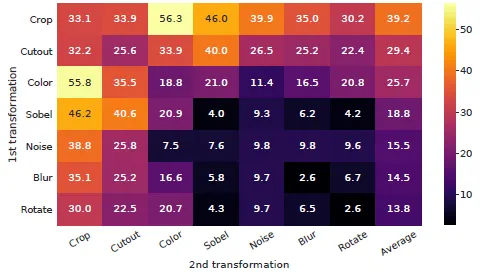
\includegraphics[scale=.5]{simCLR.png}
  \caption{Figure taken from~\cite{simCLR}. Each number corresponds to a linear evaluation of the SimCLR model using different augmentations. In the diagonal (except in average column) each transformation is only done once. For other entries, there are two augmentations done together. Higher numbers represent more accurate results. Thus the combination of crop and color distortions stands out from the rest as most benefitial augmentations \textit{for ImageNet}}
\label{fig:simCLR}
\end{figure}

% TODO: Also cite SSL section for "pulling"
One way to make \gls{SSL} work is to use distorted inputs together with the original data, e.g. in image processing this could be by rotating or cropping the image, or occluding parts of the image. It should still be possible (at least for humans) to understand what the core feature/object of the image is, otherwise the model wouldn't learn any features. SimCLR~\cite{simCLR} has a nice table (reproduced in \Cref{fig:simCLR}) to show which alterations/augmentations work better or worse than others for ImageNet. \textit{Constrastive learning} is a technique where you make a prediction on the original and modified image, and then making a loss function that can assimilate the output. Often siamese networks are used, i.e. two different models, where one model with handle the original photo and the other will handle the augmented photo. By pulling similar samples together and disjoint samples apart (by adjusting weights and biases), the model learns the important features of the image. One example of a loss function is using cosine similarity scores, where the output from each model is represented as a vector. The cosine similarity captures the angle between the vectors, and can thus be used as an indication of similarity. 

The image alterations are also called \textit{human priors}, since they rely on keeping features that humans need to understand the object. While these human priors have gotten good results on natural images, there are some domains such as medicine where they are less efficient. Especially in histopathology where there are many small details in each section of an image that are all important to make a classification. ~\cite{dataPriors} suggests to instead use \textit{data prior} for Histopathological images. One such example is using different levels of zoom as an image alteration. By zooming out, you \textit{include} more data as input. The technique works nevertheless since you want the model to focus on an area of interest (such as a tumour) regardless of its surroundings.

\section{Summary}\label{sec:summary}
Several talks that have mentioned or used new \gls{NLP} services, such as \href{ChatGPT}{https://openai.com/blog/chatgpt/} and \href{https://you.com/}{https://you.com/}. This might be an indication that \gls{NLP} has been a field with significant improvement over the last years. For \gls{DL} techniques, \gls{SSL} is mentioned in several talks (during the conference days) and seems to be popular together with constrastive learning. ImageNet is also a frequently mentioned keyword, showing the importance of big, publicly available data in general, but especially in image processing.

A common theme is that there are many pitfalls and unresolved problems in \gls{DL}. Several talks mentioned problems with lack of transferability and the generality of a model. \gls{SSL} (\Cref{sec:ssl,sec:cheese}) is dependent on its \textit{priors}. ~\Cref{sec:representative} discusses how difficult it is to find representative sample in general, and especially for training an \gls{AI}. \Cref{sec:xai} also brings up the need to ``sanity check existing sanity checks''.

% Finally, it might be important to reflect on topics that are notsome things that are \textit{not} mentioned during a \gls{DL} school are 

Finally\dots{}

\newpage

\section{Practical Project - Introduction}
\begin{comment}
The report should include both a short summary of the material covered (approx. 4 pages) and a description of the solution to a practical component.

For the practical component, you are asked to find a project that is related to one of the topics covered in the tutorials. This could for instance be self-supervised learning, where you try one of the self-supervised learning techniques on the data that you are working on in your PhD and analyse the results and or hyperparameters. Or you could take a method and evaluate its effect in new scenarios, for instance when faced with highly imbalanced data.
\end{comment}
\subsection{Background}
\dots{}summary of the paper, chatGPT maybe.


\cite{sslUMAP} uses self-supervised learning to learn morphological features of Lung Squamous Cell Carcinoma (LSCC). In training they use public TCGA and CPTAC datasets of H\&E-stained biopsy slides. They observe from previous work that other training algorithms cluster together tiles from the same slides, creating a batch effect where the algorithm learns features that are more slide specific than feature specific. This indicates that the network might do poorly on generalized input. They visualize this using 2D UMAP, shown in~\cref{fig:umap}.

\subsection{Problem Introduction}
\dots{}batches sometimes has a problem X
\dots{} They claim to have fixed the problem, but to what extent?

\section{Methodology}
\subsection{Recreating Work}
\dots{}difficult to get the code to run
\dots{}difficult to find the dataset with annotations
\dots{}difficult to find the dataset with annotations

\subsection{DataSet}

\subsection{MoCo}
\gls{MOCO}

\subsection{InceptionV4}
\dots{}

\subsection{Quantifyable explanations}\label{sec:quantifiable}
\subsubsection{Quantus}


\begin{figure}
  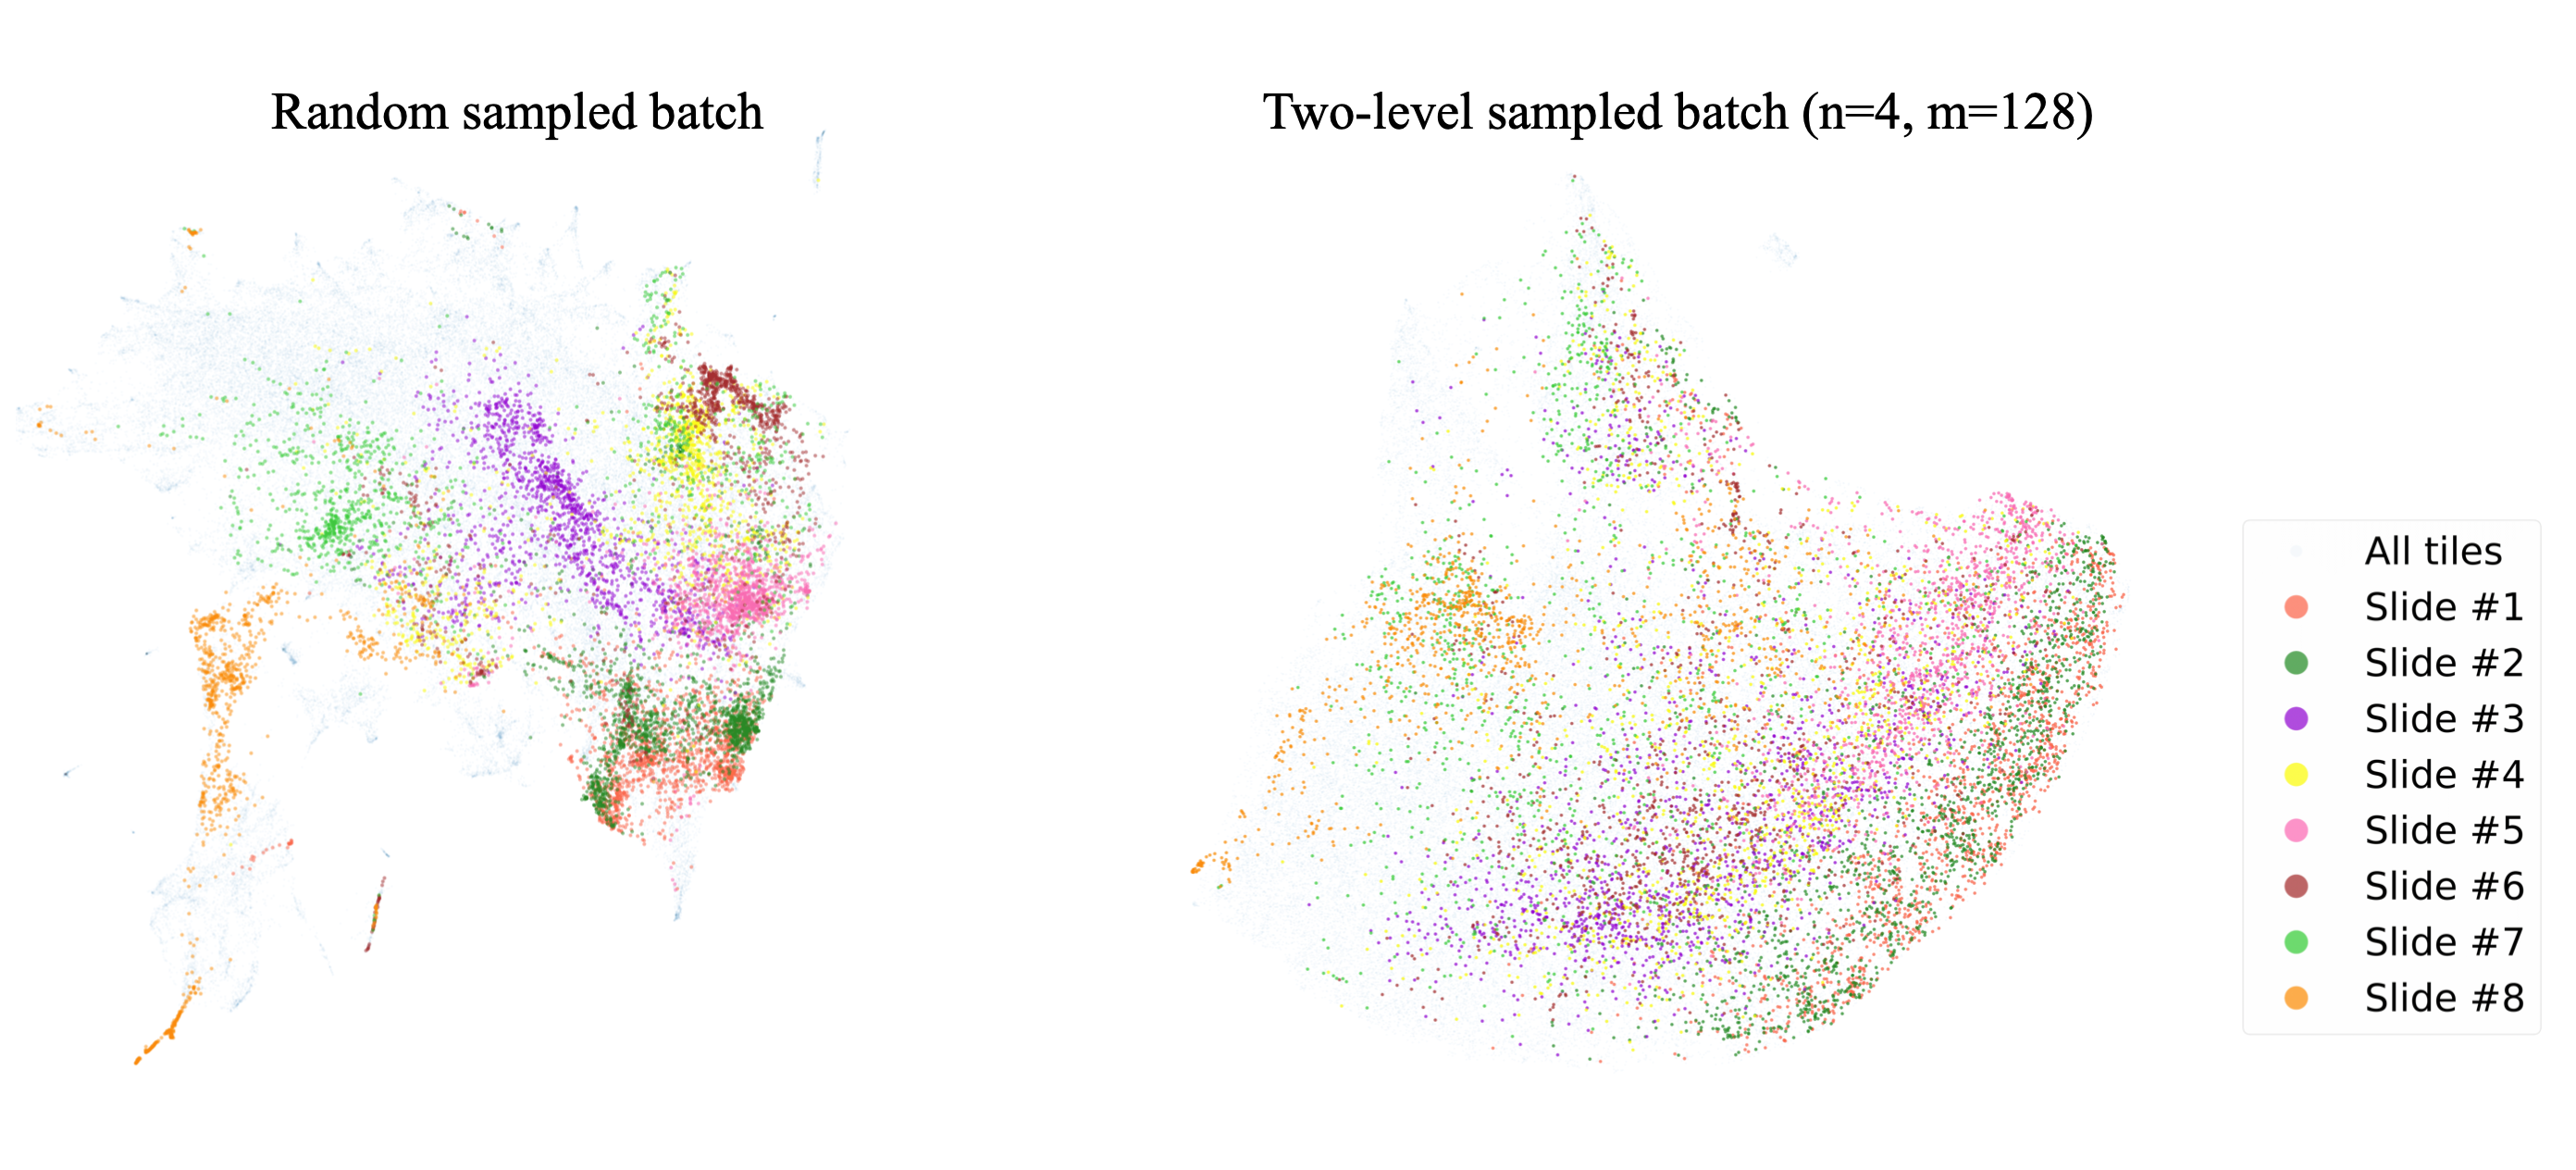
\includegraphics[scale=.17]{./umap.png}
  \caption{Figure taken entirely from~\cite{sslUMAP}. Both pictures show a 2D UMAP projection of tile representations. On the left a training algorithm with randomly sampled tiles from slides, showing that features learned in the same slide cluster together. Using a different sampling algorithm, the picture on the right shows a more even distribution w.r.t slides}
  \label{fig:umap}
\end{figure}

\subsection{UMAP}
 The algorithm is founded on three assumptions about the data
 \begin{enumerate}
   \item The data is uniformly distributed on Riemannian manifold;
   \item The Riemannian metric is locally constant (or can be approximated as such);
   \item The manifold is locally connected.
 \end{enumerate}

lack of ground truth in the data; I cannot say that two neighbors should be similar, since a model may model two samples differently even if the samples themselves are similar.

A good scoring method can indicate for each slide whether there is overlap with others; this slides is probably overfitted
A good scoring method can also average, though.
Have to keep in mind that two photos can be disparate, e.g. 1 photo can have tumours, the other can be healthy, e.g.

\subsection{Results}
\begin{table}
\centering
  \begin{tabular}{l l l l}
    Input & m1 & m2 & m3 \\
    Euclidean & 1 & 2 & 3 \\
  \end{tabular}
  \caption{Output from different sets}
  \label{tab:singleres}
\end{table}

\begin{table}
\centering
  \begin{tabular}{l l l l}
    Input & m1 & m2 & m3 \\
    Euclidean & 1 & 2 & 3 \\
  \end{tabular}
  \caption{Output from different sets}
  \label{tab:combinedres}
\end{table}

TODO: 2.9.1 Reflection in Clemmensen has a lot of stuff about metrics.

I wish to evaluate~\cite{sslUMAP} and quantify the quality of \textit{the explanation} using metrics inspired by Quantus~\cite{hedstrom2023quantus}. This means 1) finding relevant qualitative metrics for the given batch effect plots and 2) testing how the metrics change with model, batch and image adjustments. In particular, I am curious how well the metrics show batch/clustering effects for few (1-3) slides. This can be a useful indication early during a training process.

%%%%%%%%% REFERENCES
{\small
\bibliographystyle{ieee_fullname}
\bibliography{egbib}
}

\end{document}
